\documentclass[a4paper,11pt]{article}
% Various packages
\usepackage{siunitx}
\usepackage[utf8]{inputenc} % æøå
\usepackage[T1]{fontenc} % mere æøå
\usepackage[danish]{babel} % orddeling
\usepackage{verbatim} % så man kan skrive ren tekst
\usepackage{graphicx}
\graphicspath{{assets/}}
\usepackage{a4wide}
\usepackage{url}
\usepackage[left=2cm,top=2cm,bottom=1.5cm,right=2cm]{geometry}
\usepackage{amsmath}
\usepackage{amssymb}
\usepackage{amsthm}
\usepackage{wrapfig}
\usepackage{fixme}
\usepackage{color}
\usepackage{pstricks}
\usepackage{pdfpages} % include pdf
\usepackage{float} % Use [H] in figures
\usepackage{subcaption} % For subfigures
\usepackage{color} % May be necessary if you want to color links
\usepackage{hyperref} % Make references clickable
\usepackage[nameinlink,capitalize]{cleveref} % Make eq:refs be in style (1)
\usepackage[linesnumbered, commentsnumbered, lined, ruled, vlined,
%noend  % Have no ⌊-like symbol to indicate end of scope in pseudocode
]{algorithm2e} % Doc: https://goo.gl/6bC1qZ

% Ændr på navnene der vises når man bruger \autoref{label}
\def\sectionautorefname{Sektion}
\renewcommand{\equationautorefname}{Ligning}
\def\figureautorefname{Figur}
\AtBeginDocument{\renewcommand{\ref}[1]{\autoref{#1}}}

% Sæt \ref{} til at kalde \autoref{}
\AtBeginDocument{\renewcommand{\ref}[1]{\autoref{#1}}}

% Ændr ''*'' i math-felter til \cdot
\DeclareMathSymbol{*}{\mathbin}{symbols}{"01}

% Sæt farver for interne referencer og links
\definecolor{darkblue}{RGB}{25,25,112}
\hypersetup{
	colorlinks=true,    %set true if you want colored links
	linktoc=all,        %set to all if you want both sections and subsections linked
	linkcolor=darkblue, %choose some color if you want links to stand out
	filecolor=blue,     %
	citecolor=black,    %
	urlcolor=cyan,      %
}

% Set indentation to 0:
\setlength\parindent{0pt}

% Keywords relateret til algorithm2e pakken
\newcommand{\True}{\textbf{true}}\newcommand{\False}{\textbf{false}}
\SetStartEndCondition{ }{}{}%
\SetKwProg{Fn}{def}{\string:}{}
\SetKw{KwTo}{to}
\SetKwFor{For}{for}{}{}% 
\SetKwFor{ForEach}{foreach}{}{}% 
\SetKwIF{If}{ElseIf}{Else}{if}{}{elif}{else}{end}% 
\SetKwFor{While}{while}{}{end}\SetKwProg{Fn}{}{}{}
\SetKwInOut{Input}{input}\SetKwInOut{Output}{output}
\setlength{\algomargin}{3em}\DontPrintSemicolon

\newcommand{\longspace}{{\ \ \ \ \ \ \ \ \ \ \ \ \ \ }}
\renewcommand{\P}{{\mathbb P}}
\newcommand{\parfrac}[1]{\frac{\partial}{\partial #1}}
\renewcommand{\num}{{\textrm{num} }}
\newcommand{\size}{{\textrm{size} }}
\newcommand{\ift}{{\textrm{if } }}

% Dynamiske (), <>, ceil, floor
\newcommand{\p}[1]{\left( #1 \right)}
\newcommand{\pbig}[1]{\big( #1 \big)}
\newcommand{\pBig}[1]{\Big( #1 \Big)}
\newcommand{\pbigg}[1]{\bigg( #1 \bigg)}
\newcommand{\larr}[1]{\left< #1 \right>}
\newcommand{\ceil}[1]{\left\lceil #1 \right\rceil}
\newcommand{\floor}[1]{\left\lfloor #1 \right\rfloor}


% Squiggly arrows
\DeclareFontFamily{U} {MnSymbolC}{}

\DeclareFontShape{U}{MnSymbolC}{m}{n}{
	<-6> MnSymbolC5
	<6-7> MnSymbolC6
	<7-8> MnSymbolC7
	<8-9> MnSymbolC8
	<9-10> MnSymbolC9
	<10-12> MnSymbolC10
	<12-> MnSymbolC12}{}
\DeclareFontShape{U}{MnSymbolC}{b}{n}{
	<-6> MnSymbolC-Bold5
	<6-7> MnSymbolC-Bold6
	<7-8> MnSymbolC-Bold7
	<8-9> MnSymbolC-Bold8
	<9-10> MnSymbolC-Bold9
	<10-12> MnSymbolC-Bold10
	<12-> MnSymbolC-Bold12}{}

\DeclareSymbolFont{MnSyC} {U} {MnSymbolC}{m}{n}

\DeclareMathSymbol{\MNrhd}{\mathbin}{MnSyC}{76}
\DeclareMathSymbol{\MNlhd}{\mathbin}{MnSyC}{78}
% =============================================
\DeclareFontFamily{U} {MnSymbolD}{}

\DeclareFontShape{U}{MnSymbolD}{m}{n}{
	<-6> MnSymbolD5
	<6-7> MnSymbolD6
	<7-8> MnSymbolD7
	<8-9> MnSymbolD8
	<9-10> MnSymbolD9
	<10-12> MnSymbolD10
	<12-> MnSymbolD12}{}
\DeclareFontShape{U}{MnSymbolD}{b}{n}{
	<-6> MnSymbolD-Bold5
	<6-7> MnSymbolD-Bold6
	<7-8> MnSymbolD-Bold7
	<8-9> MnSymbolD-Bold8
	<9-10> MnSymbolD-Bold9
	<10-12> MnSymbolD-Bold10
	<12-> MnSymbolD-Bold12}{}

\DeclareSymbolFont{MnSyD} {U} {MnSymbolD}{m}{n}
\DeclareMathSymbol{\MNsim}{\mathbin}{MnSyD}{2}

% =============================================

\usepackage{amssymb,amsmath,stackengine}
\stackMath
\newcommand\rsquigarrow[1]{%
	\mathbin{\stackon[2pt]{\rightsquigarrow}{\scriptscriptstyle #1 }}
}

\author{Søren Mulvad, rbn601}

\title{Eksamensdisposition - Amortiseret analyse}
\begin{document}
\maketitle

% Desuden skal hver studerende i gruppen udarbejde en individuel disposition for emnet "Binære søgetræer", som er et af emnerne til eksamen. En disposition skal bestå af de vigtigste punkter, du vil komme ind på til eksamen.
% Tænk på dispositionen som noget, du kan have med dig til eksamen, og som kan hjælpe dig med at huske, hvad du overordnet vil gennemgå til emnet "Binære søgetræer".
% Dispositionen skal ikke indeholde detaljerede beviser og lignende, men de mere overordnede delemner. Sørg for at gøre den kortfattet - f.eks. 5-10 punkter med stikord/-sætninger.


\begin{itemize}
\item \textbf{Motivation}

\item \textbf{Aggregeret analyse}
\begin{itemize}
	\item Stack-eksempel
\end{itemize}

\item \textbf{Accounting method}
\begin{itemize}
	\item Stack-eksempel
\end{itemize}


\item \textbf{Potentiale metode}
\begin{itemize}
	\item Generelt
	\item Stack-eksempel
	\item Dynamisk tabel kun med \texttt{Insert}
\end{itemize}


\end{itemize}

%%%%%%%%%%%%%%%%%%%%%%%%%%%%%%%%%%%%%%%%%%%%%%%%%%%%%%%%%%%
%%%%%%%%%%%%%%%%%%%%%%%%%%%%%%%%%%%%%%%%%%%%%%%%%%%%%%%%%%%
%%%%%%%%%%%%%%%%%%%%%%%%%%%%%%%%%%%%%%%%%%%%%%%%%%%%%%%%%%%
\newpage
%%%%%%%%%%%%%%%%%%%%%%%%%%%%%%%%%%%%%%%%%%%%%%%%%%%%%%%%%%%
%%%%%%%%%%%%%%%%%%%%%%%%%%%%%%%%%%%%%%%%%%%%%%%%%%%%%%%%%%%
%%%%%%%%%%%%%%%%%%%%%%%%%%%%%%%%%%%%%%%%%%%%%%%%%%%%%%%%%%%
\section{Amortiseret analyse}



\begin{itemize}
\item \textbf{Motivation}
\begin{itemize}
	\item Nogle gange er vi for en datastruktur ikke interesseret i dens worst case køretid hver eneste gang en operation udføres, men i stedet interesseret i hvad average case er når vi udfører en række af instruktioner.
	\item Jeg vil her illustrere koncepterne på nogle lidt tænkte eksempler, men amortiseret analyse er også relevant i Fibonacci Heaps, og dermed i Dijkstras algoritme og Prims algoritme (MST), samt i disjoint-set forests hvilket benyttes i Kruskals algoritme (MST).
\end{itemize}


\item \textbf{Aggregeret analyse}
\begin{itemize}
	\item Antag vi har en stack der har operationerne \texttt{Push(S, x)}, \texttt{Pop(S)}, \texttt{Stack-Empty(S)} som alle tager $\Theta(1)$-tid.\\
	Derudover har vi \texttt{MultiPop(S, k)}, som kalder \texttt{Pop} og \texttt{Stack-Empty} et antal gange der svarer til minimum af antal elementer og en parameter $k$ vi giver den. Denne vil køre i $\Theta(\min(s, k))$-tid.
	\item Hvis vi udfører $n$ operationer på en stack der til at starte med er tom ser vi, at vi worst-case får en køretid på $O(n^2)$.
	\item Vi beregner et upper bound $T(n)$ for alle $n$ operationer og får derved den amortiserede cost pr. operation til $T(n)/n$.
	\item Nu udnytter vi, at der højest kan være $n$ \texttt{Push}-operationer og der kan ikke være flere \texttt{Pop}-operationer (inklusiv dem i \texttt{MultiPop}) end \texttt{Push}-operationer.
	\item Så får vi at worst-case for alle $n$ operationer er $O(n)$, og herved at den amortiserede cost pr. operaton er $O(n)/n = O(1)$.
\end{itemize}

\item \textbf{Accounting method}
\begin{itemize}
	\item Den rigtige cost for den $i$'te operation er $c_i$\\
	Den amortiserede cost for den $i$'te operation er $\hat c_i$.
	\item Hvis $\hat c_i > c_i$, så overcharger vi operationen og har på den måde noget ''kredit'' at bruge af. Hvis det omvendte gør sig gældende, så undercharger vi og bruger herved noget af den kredit vi har bygget op.
	\item Der skal ALTID gælde:
	$$
	\sum_{i=1}^n c_i \leq \sum_{i=1}^n \hat c_i
	$$
	Hvis vi nu kan få et upper bound på $\sum_{i=1}^n \hat c_i$ får vi også et upper bound på den faktiske omkostning.
	\item Nu henholdsvis får/vælger vi følgende værdier:
	\begin{table}[H] \begin{center}
		\begin{tabular}{l|c|l}
			\textbf{Operation} & \textbf{Faktisk cost} & \textbf{Amortiseret cost} \\ \hline
			\texttt{Push}      & $1$                   & $2$                       \\
			\texttt{Pop}       & $1$                   & $0$                       \\
			\texttt{MultiPop}  & $\min(s, k)$          & $0$
		\end{tabular} \end{center}
	\end{table}
	Vi kan se på det på den måde, at ved \texttt{Push} betaler vi både for selve operationen med 1 samt lægger 1 kredit på elementet.
	\item \texttt{Pop} bliver undercharged med 1, men denne cost betaler vi med den kredit vi har lagt på elementet. Vi ser at vi aldrig får en kredit der er negativ.
	\item Vi ser, at for enhver sekvens af $n$ operationer har vi
	$$
	\sum_{i=1}^n c_i \leq \sum_{i=1}^n \hat c_i \leq 2n
	$$
	og herved bliver den gennemsnitlige cost $\leq 2$, hvorved vi får en gennemsnitlig køretid på $O(1)$.
\end{itemize}





\item \textbf{Potentialemetoden - Generelt}
\begin{itemize}
	\item Minder lidt om accounting method bortset fra at kreditten ikke er gemt på enkelte elementer men i stedet i ''banken''. Mængden af kredit i banken er udtrykt ved en potentialefunktion $\Phi$.
	\item Hvis vi udfører $n$ operationer på en datastruktur hvor $D_i$ er strukturen efter den $i$'te operation for $i = 1, ..., n$, så skriver vi $\Phi(D_i)$ som symbol for kreditten der er gemt med den nuværende struktur.
	\item Vi definerer den amortiserede cost $\hat c_i$ som den faktiske cost $c_i$ plus forskellen mellem hvad der er i potentialet nu og hvad der var lige før.
	$$
	\hat c_i = c_i + \Phi(D_i) - \Phi(D_{i-1})
	$$
	Hvis $\Phi(D_i) - \Phi(D_{i-1}) > 0$ kan man sige at vi putter kredit i banken, og hvis det er mindre tager vi kredit fra banken.
	\item Samme egenskab som for accounting method skal gælde:
	\begin{equation} \label{eq:ineq}
	\sum_{i=1}^n \hat c_i \geq \sum_{i=1}^n c_i
	\end{equation}
	\item Vi får summen af den amortiserede cost til at blive:
	\begin{align*}
	\sum_{i=1}^n \hat c_i &= \sum_{i=1}^n \pBig{ c_i + \Phi(D_i) - \Phi(D_{i-1}) }\\
	&= c_1 + \Phi(D_1) - \Phi(D_0)\\
	&+ c_2 + \Phi(D_2) - \Phi(D_1)\\
	&+ \vdots\\
	&+ c_n + \Phi(D_n) - \Phi(D_{n-1})\\
	&= \p{ \sum_{i=1}^n c_i } + \Phi(D_n) - \Phi(D_0)
	\end{align*}
	Da vi ser at alle potentiale-led pånær det første og sidste går ud med hinanden i summen. Hvis vi sørger for at $\Phi(D_n) \geq \Phi(D_0)$ ser vi, at vi vil opfylde \cref{eq:ineq}.
\end{itemize}

\item \textbf{Potentialemetoden - Stack-eksempel}
\begin{itemize}
	\item Vi vælger en potentialefunktion $\Phi(D_i)$ = antallet af elementer på stacken.\\
	Vi ser tydeligt at \cref{eq:ineq} er overholdt, da $D_0 = 0$ og $\Phi(D_i) \geq 0$ for alle $i$.
	\item Nu skal vi upper bound'e dette.
	\item \texttt{Push}:
	\begin{itemize}
		\item $\Phi(D_i) - \Phi(D_{i-1}) = 1$ (der tilføjes et element til stacken)
		\item Derved fås $\hat c_i = c_i + \Phi(D_i) - \Phi(D_{i-1}) = 1+1 = 2$
	\end{itemize}
	\item \texttt{Pop}:
	\begin{itemize}
		\item $\Phi(D_i) - \Phi(D_{i-1}) = -1$ (der fjernes et element fra stacken)
		\item Derved fås $\hat c_i = c_i + \Phi(D_i) - \Phi(D_{i-1}) = 1-1 = 0$
	\end{itemize}
	\item \texttt{MultiPop}:
	\begin{itemize}
		\item Lad os sige vi popper $k' > 0$ elementer.
		\item $\Phi(D_i) - \Phi(D_{i-1}) = -k'$ (da der fjernes $k'$ elementer fra stacken)
		\item Derved fås $\hat c_i = c_i + \Phi(D_i) - \Phi(D_{i-1}) = k' - k' = 0$
	\end{itemize}
	\item For alle operationer $i = 1, ..., n$ gælder, at $\hat c_i \leq 2$. Herved får vi følgende ulighed:
	$$
	\sum_{i=1}^n c_i \leq \sum_{i=1}^n \hat c_i \leq 2n
	$$
	Og derved er den gennemsnitlige tid brugt pr. operation $2n/n = O(1)$.
\end{itemize}


\item \textbf{Potentialemetoden - Dynamisk tabel kun med \texttt{Insert}}
\begin{itemize}
	\item Nu indfører vi en abstrakt datastruktur $T$, som vi kan tænke på som en tabel. Den understøtter \texttt{Insert} og \texttt{Delete}, bruger et array til at gemme sin data og bruger $O(k)$ tid på at allokere/free'e et array af størrelse $k$. For nu antager vi, at $T$ kun understøtter \texttt{Insert}.
	\item Vi ønsker at $T$ dynamisk allokerer et nyt større array til sig selv når det gamle array er for småt til at indeholde alle elementerne.
	\item Indfør følgende notation:
	\begin{itemize}
		\item $\num_i$: Antallet af elementer i $T$ efter den $i$'te operation
		\item $\size_i$: Størrelsen af arrayet for $T$ efter den $i$'te operation
		\item $\alpha_i = \num_i / \size_i$, loadfaktoren af $T$ efter den $i$'te operation (hvis $\size_i = 0$, definer $\alpha_i = 1$). 
	\end{itemize}
	\item Vi starter med at $T$ er tom. Herefter siger vi, at lige før vi indsætter det $i$'te element, hvis $\num_{i-1} = \size_{i-1}$ (svarende til loadfaktoren $\alpha_{i-1} = 1$) så ekspanderer vi $T$ til et array der er dobbelt så stort, $2 \size_{i-1}$ og kopierer de gamle elementer over.
	\item Vi ser at tabelekspandering tager $O(\num_i)$ worst-case tid. Så hvis den $i$'te operation kræver en ekspandering kan vi sætte $c_i = \num_i$.
	\item Hvis ingen ekspandering er krævet kan vi sætte $c_i = 1$.\\
	
	\item Definer potentialefunktionen
	$$
	\Phi(D_i) = 2 \num_i - \size_i
	$$
	\begin{figure}[H]
		\begin{center}
			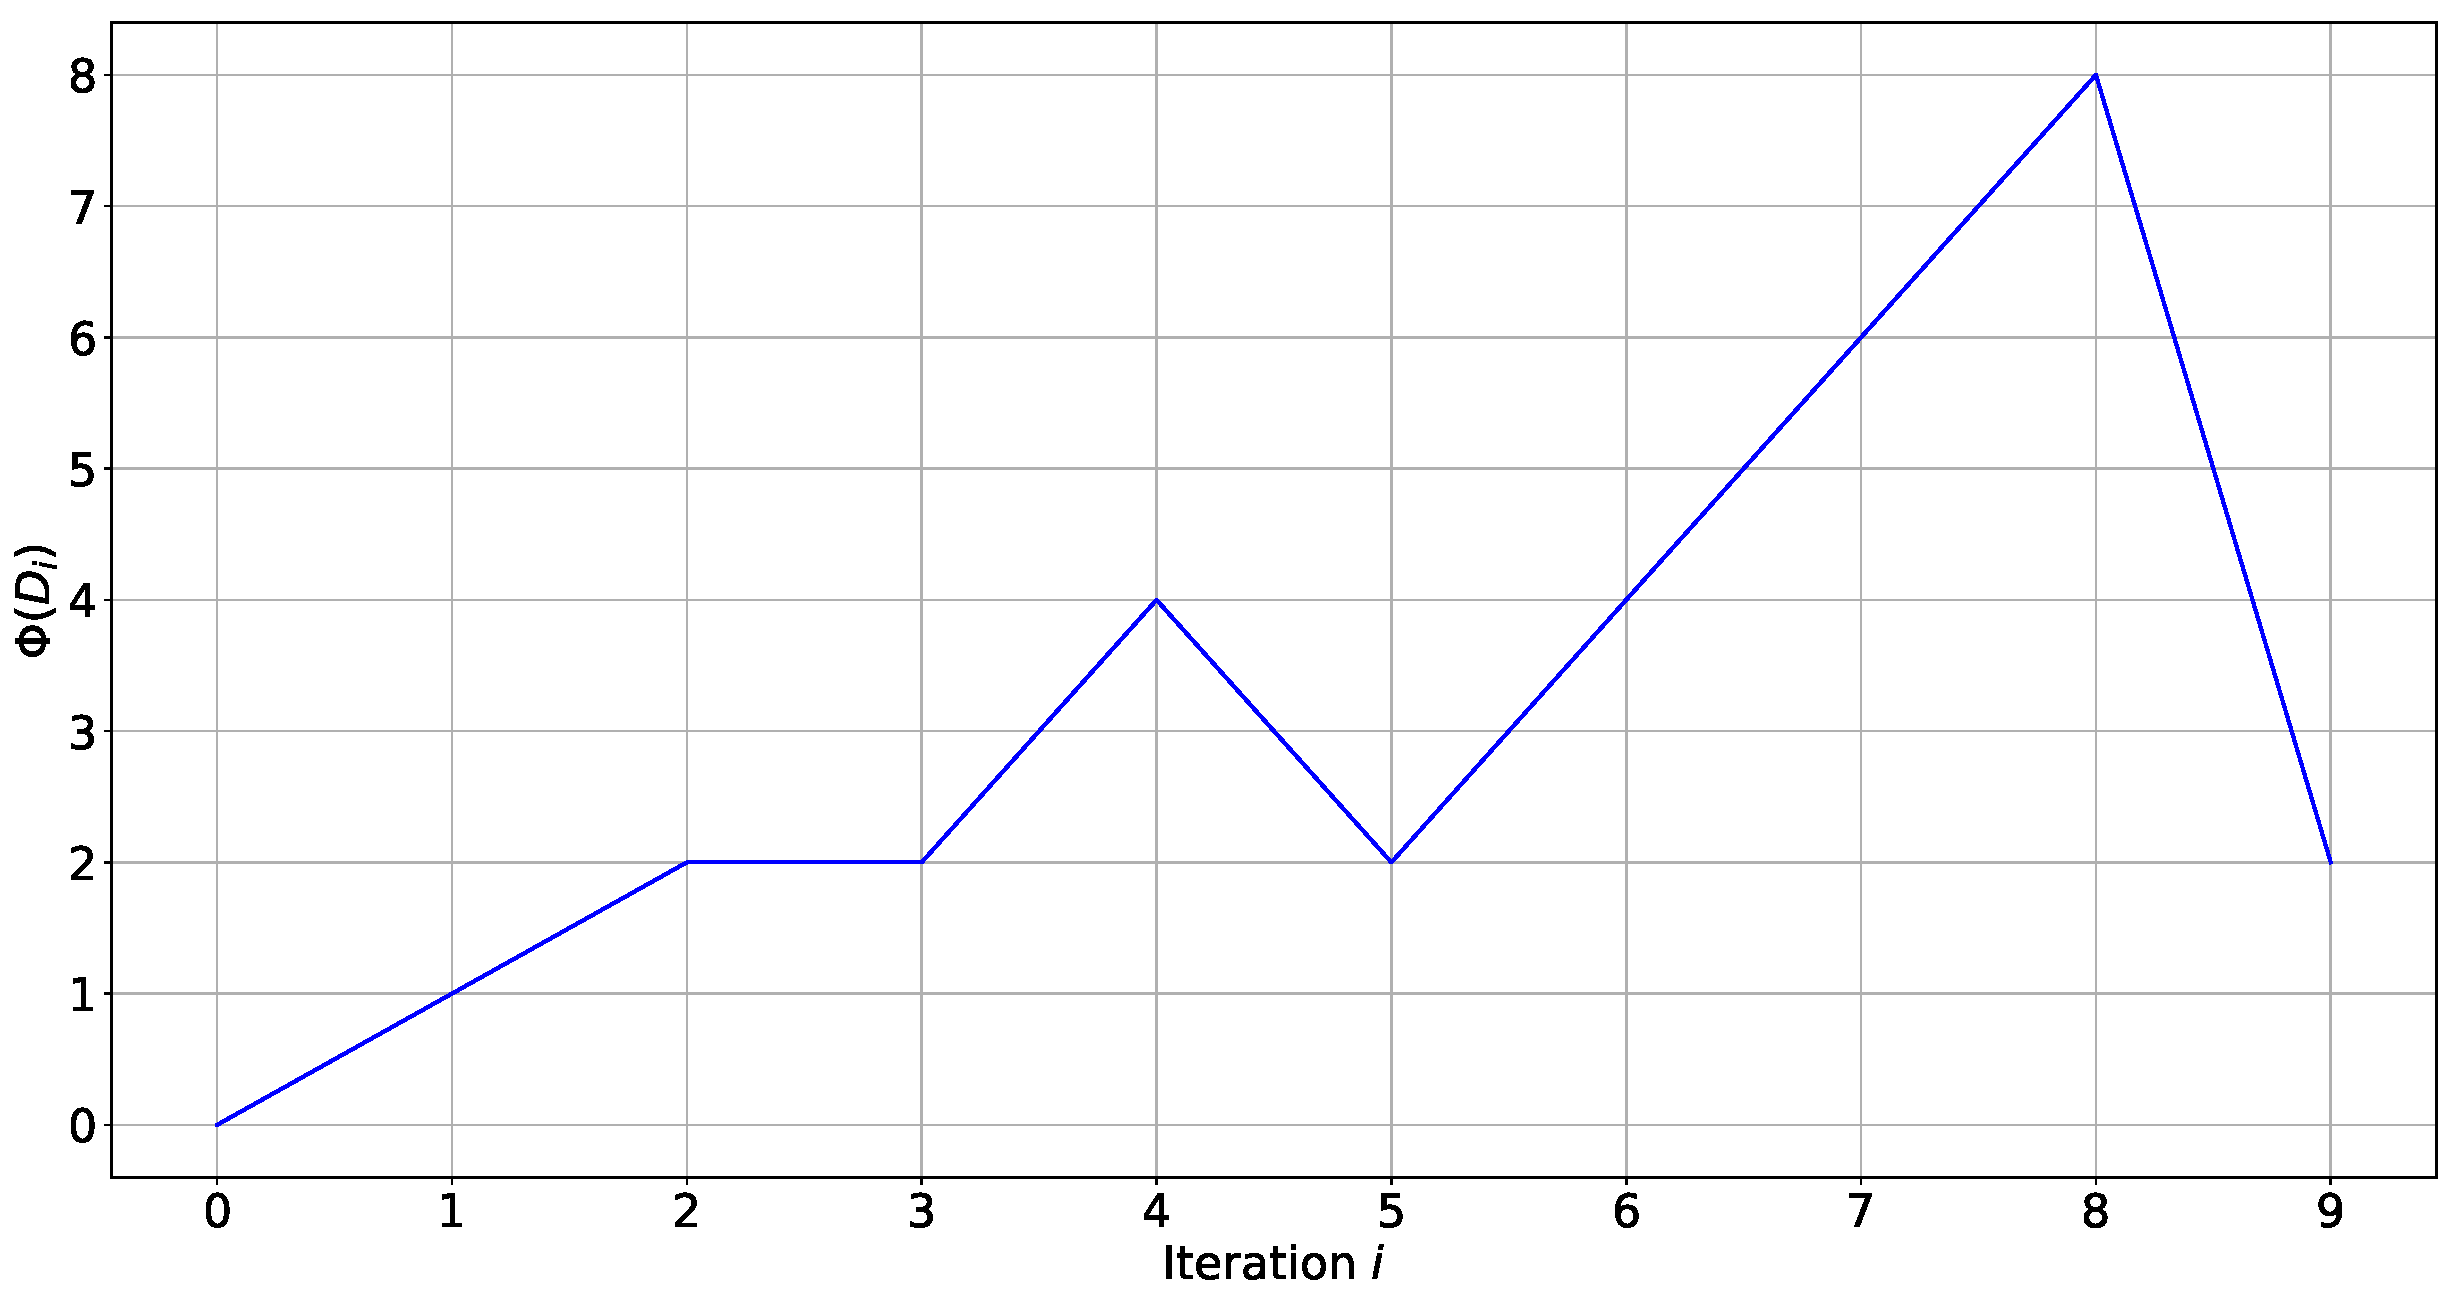
\includegraphics[width=0.8\textwidth]{potential.pdf}
		\end{center}
		\caption{Potentialet $\Phi(D_i)$ efter hver iteration $i$}
		\label{fig:pot}
	\end{figure}
	\item Først vis den er valid ved at vise $\Phi(D_0) = 0$ og $\Phi(D_i) \geq 0$ for alle $i$.
	\item Tydeligvis er $\Phi(D_0) = 0$ da $T$ er tom til at starte med. Og da vi har, at $T$ altid som minimum er halvt fyld, så har vi også $\Phi(D_i) \geq 0$ for alle $i$. Derfor gælder \cref{eq:ineq}.
	\item Da \cref{eq:ineq} gælder kan vi få et upper bound for $\sum_{i=1}^n c_i$ ved at upper bound'e $\sum_{i=1}^n \hat c_i$.
	\item Hvis der IKKE sker tabelekspandering får vi følgende amortiserede cost:\\
	\begin{align*}
	\hat c_i &= c_i + \Phi(D_i) - \Phi(D_{i-1})\\
	         &= 1 + (2 \num_i - \size_i) - (2 \num_{i-1} - \size_{i-1})\\
	         &= 1 + (2 \num_i - \size_i) - (2(\num_i - 1) - \size_i)\\
	         &= 3
	\end{align*}
	Vi får dette da size ikke ændrer sig, og det forrige antal elementer svarer til det nuværende antal elementer minus en, da vi jo netop har tilføjet en. 3-tallet fås ved at se, at ting går ud med hinanden.
	\item Hvis der SKER tabelekspandering OG $i = 1$ får vi den amortiserede cost 2.
	\item Hvis der SKER tabelekspandering OG $i > 1$ får vi:
	%\begin{figure}[H]
		\begin{center}
			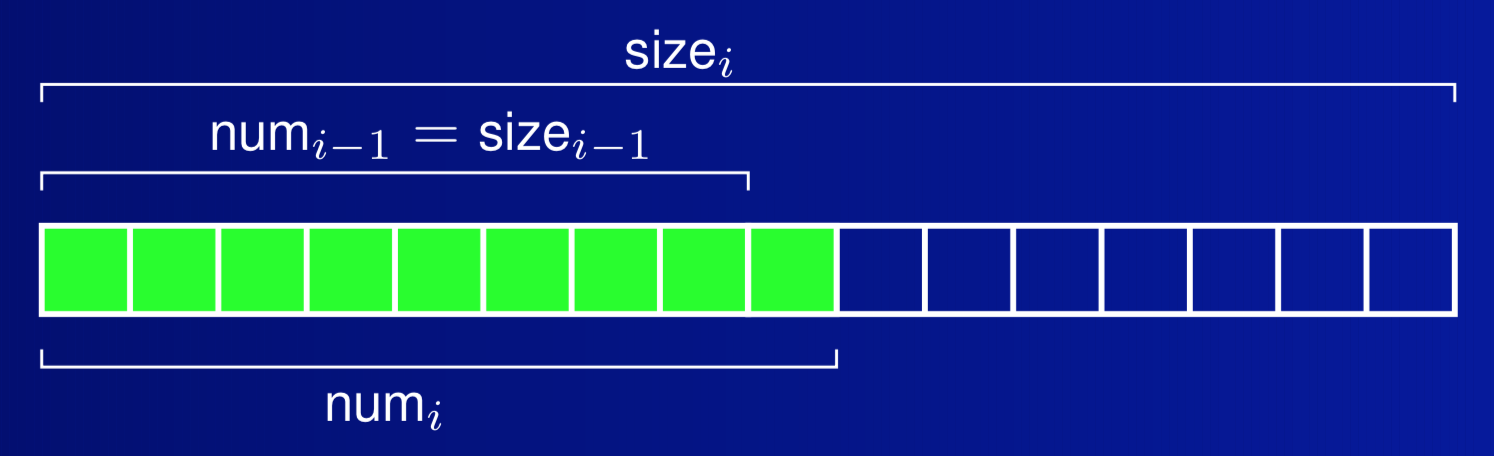
\includegraphics[width=0.8\textwidth]{ekspandering.png}
		\end{center}
	%	\caption{caption}
	%	\label{fig:insert-table}
	%\end{figure}
	\begin{align*}
	\hat c_i &= c_i \Phi(D_i) - \Phi(D_{i-1})\\
	         &= \num_i + \p{2\num_i - \size_i} - \p{2\num_{i-1} - \size_{i-1}}\\
	         &= \num_i + \pBig{2\num_i - 2(\num_i - 1)} - \pBig{2(\num_i - 1) - (\num_i - 1)}\\
	         &= 3
	\end{align*}
	\textit{Hvordan disse numre fås kan ræsonneres ud fra grafen, bare husk at alle variabler skal være} $\num_i$ \textit{til sidst.}
\end{itemize}

\item \textbf{Potentialemetoden - High-level bevis når vi har \texttt{Insert}/\texttt{Delete}}
\begin{itemize}
	\item Forklaring af \texttt{Delete}: Vi ønsker at kunne fjerne elementer fra tabellen igen, og såfremt vi når ned under en hvis loadfaktor $\alpha_i$ at bruge et mindre array til at holde dem. Naiv implementation vil være at gå til mindre array når $\alpha_i < 1/2$, men så kunne vi potentielt få et problem hvis vi indsætter og sletter mange gange meget tæt på en 2-tals potens.
	\item I stedet vælger vi at gøre det når vi når ned under en loadfaktor $\alpha_i < 1/4$, og så kan man faktisk vise at vi understøtter \texttt{Insert} og \texttt{Delete} i $O(1)$ amortiseret tid.
	\item Vi vælger nu potentialemetoden:
	\begin{align}
	\Phi(D_i) =
	\begin{cases}
	2 \num_i - \size_i   & \ift \alpha_i \geq 1/2\\
	\size_i / 2 - \num_i & \ift \alpha_i < 1/2
	\end{cases} \label{eq:pot2}
	\end{align}
	Da får vi følgende graf:
	\begin{figure}[H]
		\begin{center}
			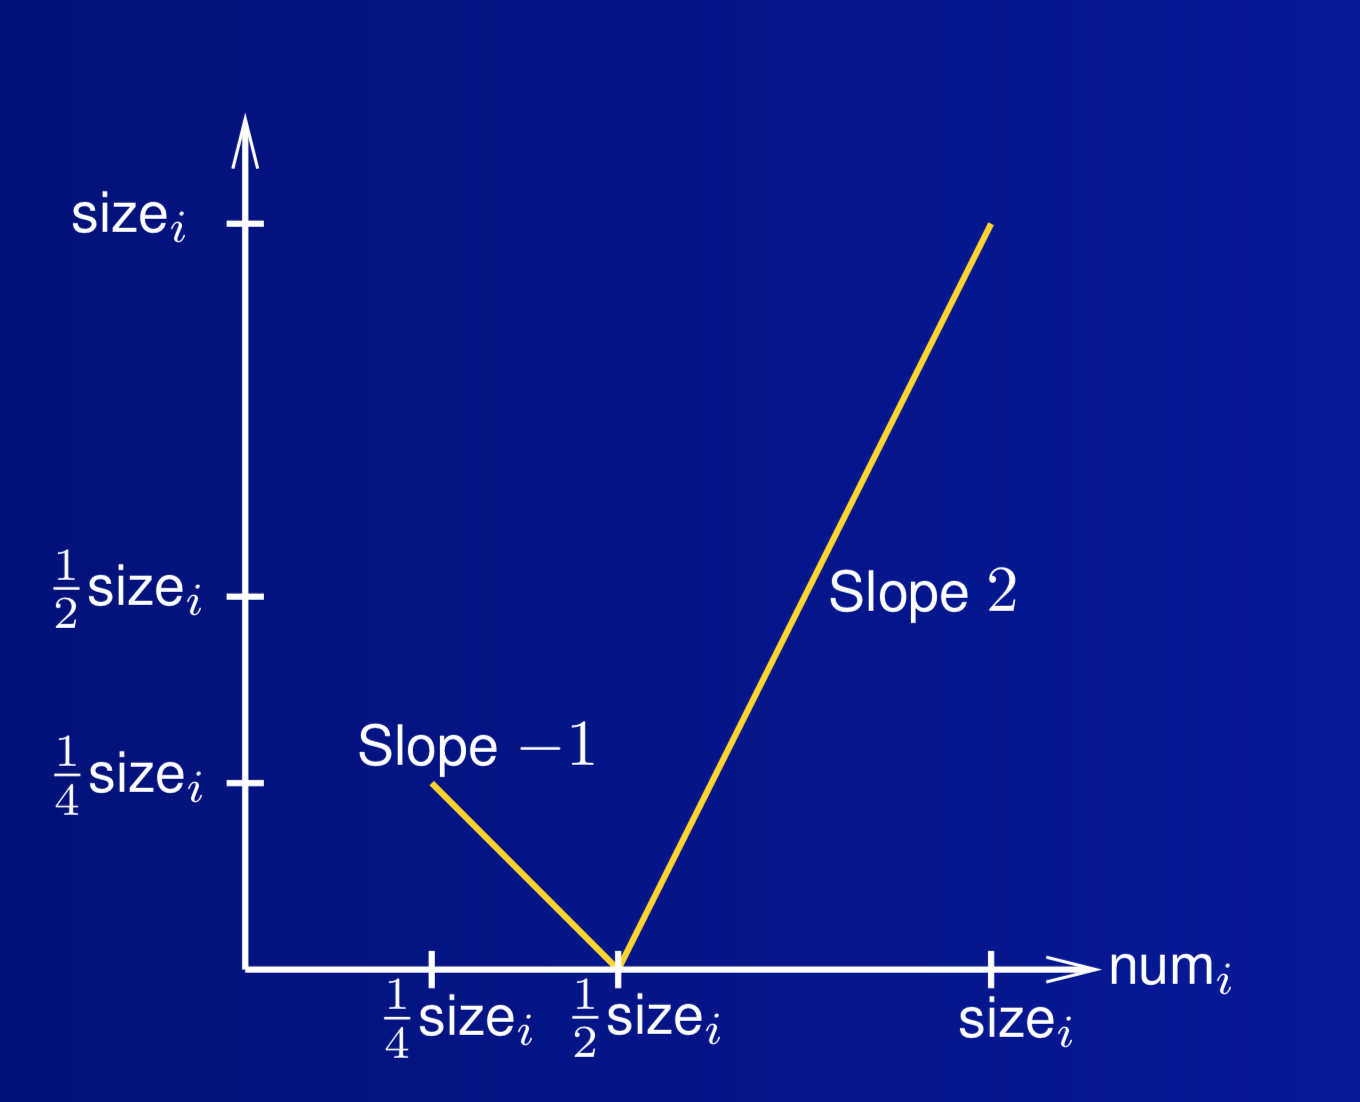
\includegraphics[width=0.5\textwidth]{delete.png}
		\end{center}
		\caption{Hvordan grafen vokser}
		\label{fig:delete}
	\end{figure}

	\item Vi observerer, at lige før en tabel ekspandering/forkortelse har $\Phi$ værdien $\num_i$. Lige efter er tabellen cirka halv fuld og derfor dropper potentialet til omkring $0$. Dette drop i potentiale ''betaler'' for ekspanderingen/forkortelsen.
	\item Når der ikke sker en ekspandering/forkortelse, så er den amortiserede cost højest 3 siden den absolutte hældning af $\Phi$ højest er 2.
	
\end{itemize}


\item \textbf{Potentialemetoden - Bevis for amortiseret cost af \texttt{Delete}}
\begin{itemize}
	\item Hvis der ikke sker nogen tabelforkortelse, så kan vi ud fra grafen argumentere for, at $\hat c_i \leq 2$ da $c_i = 1$.
	\item Hvis der SKER en tabelforkortelse, så vil ét element slettes og $\num_i$ elementer flyttes til det forkortede array, så den faktiske cost er $c_i = \num_i + 1$. Vi har at loadfaktoren vil være under $1/2$ for både før og efter operationen, så vi bruger case 2 i \cref{eq:pot2} for begge.
	\item Da får vi:
	\begin{center}
		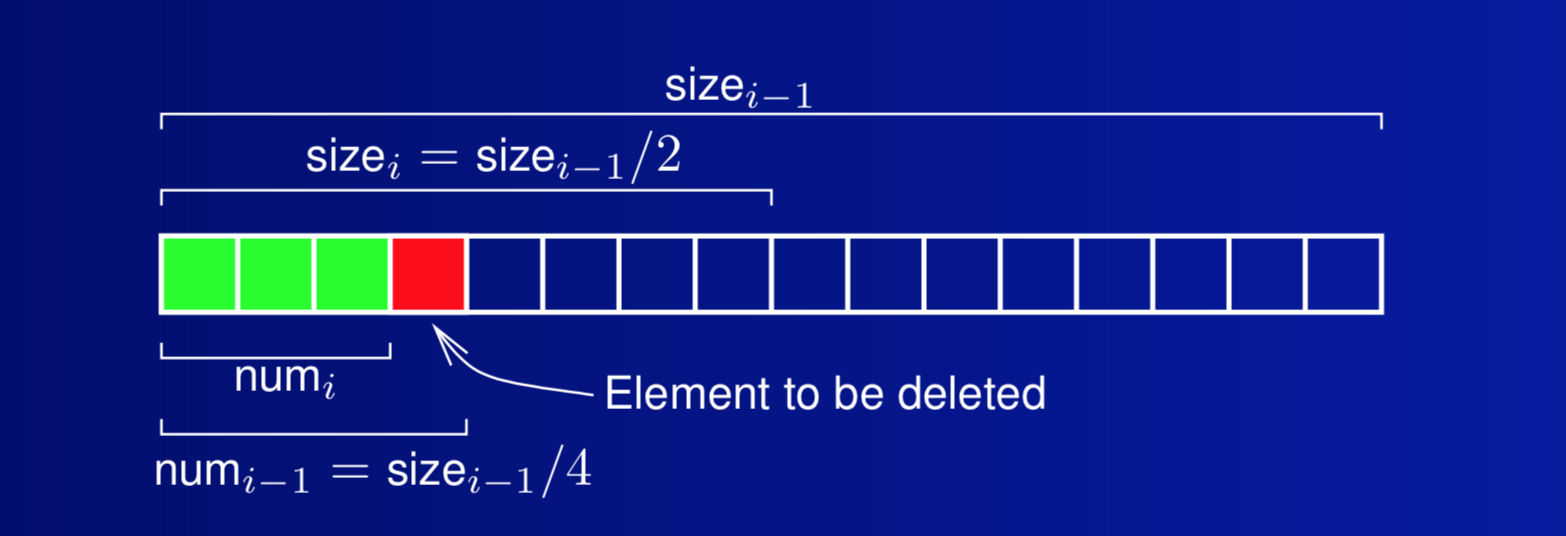
\includegraphics[width=0.8\textwidth]{del2.png}
	\end{center}
	\begin{align*}
	\hat c_i &= c_i + \Phi(D_i) - \Phi(D_{i-1})\\
	         &= \num_i + 1 + \p{ \size_i / 2 - \num_i } - \p{ \size_{i-1} / 2 - \num_{i-1} }\\
	         &= \num_i + 1 + \p{ (\num_i + 1) - \num_i } - \p{ 2(\num_i + 1) - (\num_i + 1) }\\
	         &= 1
	\end{align*}
	\textit{Husk igen på at vi skal have} $\num_i$ \textit{som eneste variabel, og ræsonner da ud fra figuren.}
\end{itemize}


\end{itemize}
\end{document}